% !TeX spellcheck = en_US
% !TEX root = ../thesis-example.tex
%
\newpage
\section{Mitigating Frame Jitter}
\label{sec:framejitter}

An additional step that can be handled by the same algorithm is the mitigation 
of frame or time jittering, a term describing an effect of different running 
framerates of an actor's captured video footage and rate of 3D environment 
rendering. Since the native framerate of the HMD is higher than the frames 
produced by the input video feed, there will be noticeable small jitters of 
virtual camera movement, which are not present on the source video material. 
The HTC Vive Controllers are very good at picking up minuscule changes in 
motion, which are instantly translated to the transform matrix on the virtual 
camera rig and then yield minor motion of the 3D environment projection. 
Visually this shows in a shaking virtual world while the real world video 
stands still.

To minimize the effect, it is possible to overwrite \code{Render Textures} for 
as long as one duration of a video frame and then forward swapping out these 
buffers. The headset recommends to run it at 90fps and mistiming is no 
issue either, since it results in non-noticeable errors in virtual projections 
while the displayed frame is stable, thus visual performance of the 
presentation device is unaffected. It is possible to write less than three 
times into a \code{Render Textures}, which is mitigated again by displaying the 
final result later --- the composed image is therefore unaffected besides 
imperceptible differences between the real world camera and its virtual 
transformation matrix.

\begin{figure}[htb]
	\centering
	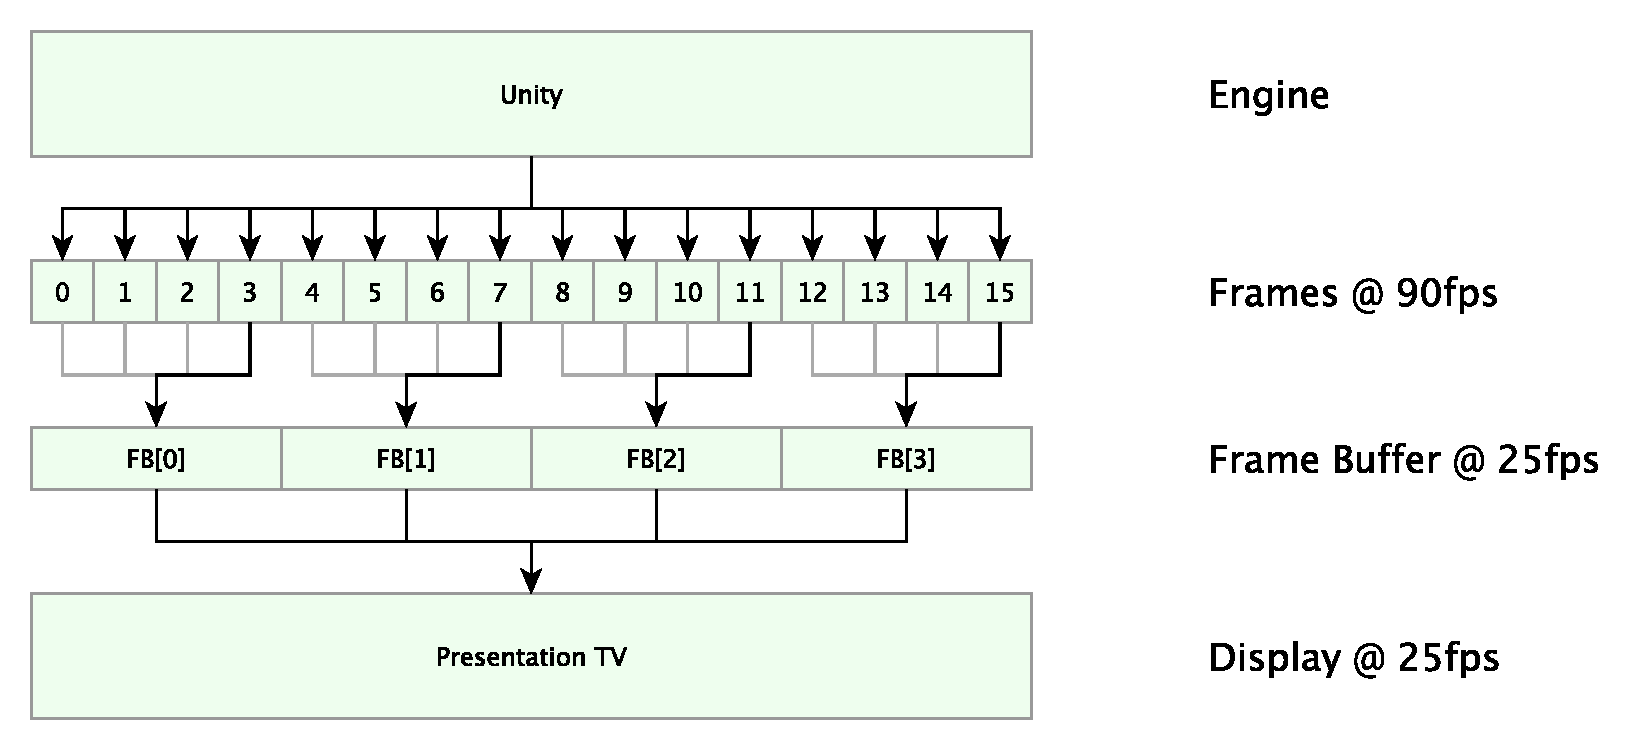
\includegraphics[width=\textwidth]{gfx/Delay_Mitigation.pdf}
	\caption{Workflow of the render swapper, in which rendered frames will be 
		overwritten as long as it is needed - and then another frame buffer 
		will be written into.}
	\label{fig:offsets:framesquashing}
\end{figure}
